\documentclass[17pt]{beamer}
%\documentclass[aspectratio=169,17pt]{beamer}

\mode<presentation>
\usetheme[height=-8pt]{Waterloo}

%%%%%%%%%%%%%
%% OPTIONS %%
%%%%%%%%%%%%%

% make whale theme super striking
\setbeamercolor*{frametitle}{parent=palette primary}

% make whale theme more subtle
%\setbeamercolor*{block title}{use=structure,fg=black,bg=structure.fg}

% by default dark titles; change to light with
%\usecolortheme{seahorse}
%\usecolortheme{rose}

% navigation symbols are lame; get rid with
\setbeamertemplate{navigation symbols}{}

% use serifs for math (kind of necessary)
\usefonttheme[onlymath]{serif}

%%%%%%%%%%%%%%%%%%%%%%%%%%
%% NO MORE REAL OPTIONS %%
%%%%%%%%%%%%%%%%%%%%%%%%%%

\usepackage{graphicx}
\usepackage{booktabs}
\usepackage{minted}
\usepackage[T1]{fontenc}
%\usepackage{textcomp}
\usepackage{futura}
% \usepackage{helvet}  % Futura is a pain to install...
\usepackage{inconsolata}

% Center a figure
\newcommand{\cf}[2]{
    \begin{center}
      \includegraphics[width=#2\columnwidth]{#1}
    \end{center}
  }

\graphicspath{{../figures/}}
\newcommand*\mystrut[2]{\vrule width0pt height#1pt depth#2pt\relax}

% Minted stuff
\makeatletter
\renewcommand\minted@pygmentize[2][\jobname.pyg]{
  \def\minted@cmd{pygmentize -l #2 -f latex -F tokenmerge
    \minted@opt{gobble} \minted@opt{texcl} \minted@opt{mathescape}
    \minted@opt{startinline} \minted@opt{funcnamehighlighting}
    \minted@opt{linenos} -P "verboptions=\minted@opt{extra}"
    -O stripnl=false -o \jobname.out.pyg #1}
  \immediate\write18{\minted@cmd}
  \ifthenelse{\equal{\minted@opt@bgcolor}{}}
   {}
   {\begin{minted@colorbg}{\minted@opt@bgcolor}}
  \input{\jobname.out.pyg}
  \ifthenelse{\equal{\minted@opt@bgcolor}{}}
   {}
   {\end{minted@colorbg}}
  \DeleteFile{\jobname.out.pyg}}
\makeatother

%%%%%%%%%%%%%%%%%%%%%%%
%% PRESENTATION INFO %%
%%%%%%%%%%%%%%%%%%%%%%%
\title{Writing self-documenting scientific code \\ using physical quantities}
\author{Trevor Bekolay}
\institute{Center for Theoretical Neuroscience \text{@} University of Waterloo}
\date{\footnotesize \url{https://github.com/tbekolay/pyconca2012}}

%%%%%%%%%%%%%%%%%%
%% PRESENTATION %%
%%%%%%%%%%%%%%%%%%
\begin{document}

\frame[plain]{\titlepage}

\begin{frame}
  \vspace{-32pt}
  \begin{huge}
    \begin{equation*}
      \overbrace{\text{v = }
        \underbrace{\mystrut{44}{20} \text{35.0}}_\text{\large Magnitude}
        \text{ }
        \underbrace{\mystrut{44}{20} \text{m/s}}_\text{\large Unit}
      }^\text{\large Quantity}
    \end{equation*}
  \end{huge}
\end{frame}

\begin{frame}
  \vspace{-12pt}
  \cf{mars_orbiter}{0.65}
\end{frame}

\begin{frame}
  \vspace{-12pt}
  \hspace*{-.055\columnwidth}
  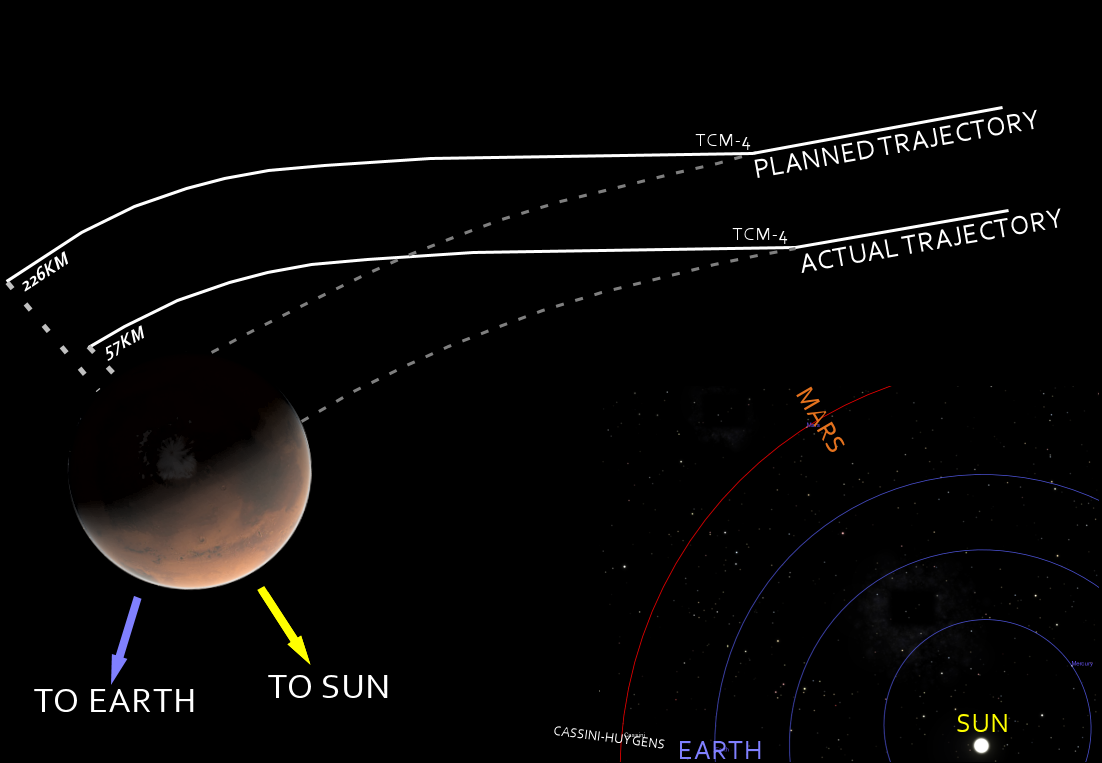
\includegraphics[width=1.1\columnwidth]{mars_orbiter_mishap}
\end{frame}

\begin{frame}
  \vspace{-12pt}
  \hspace*{-.055\columnwidth}
  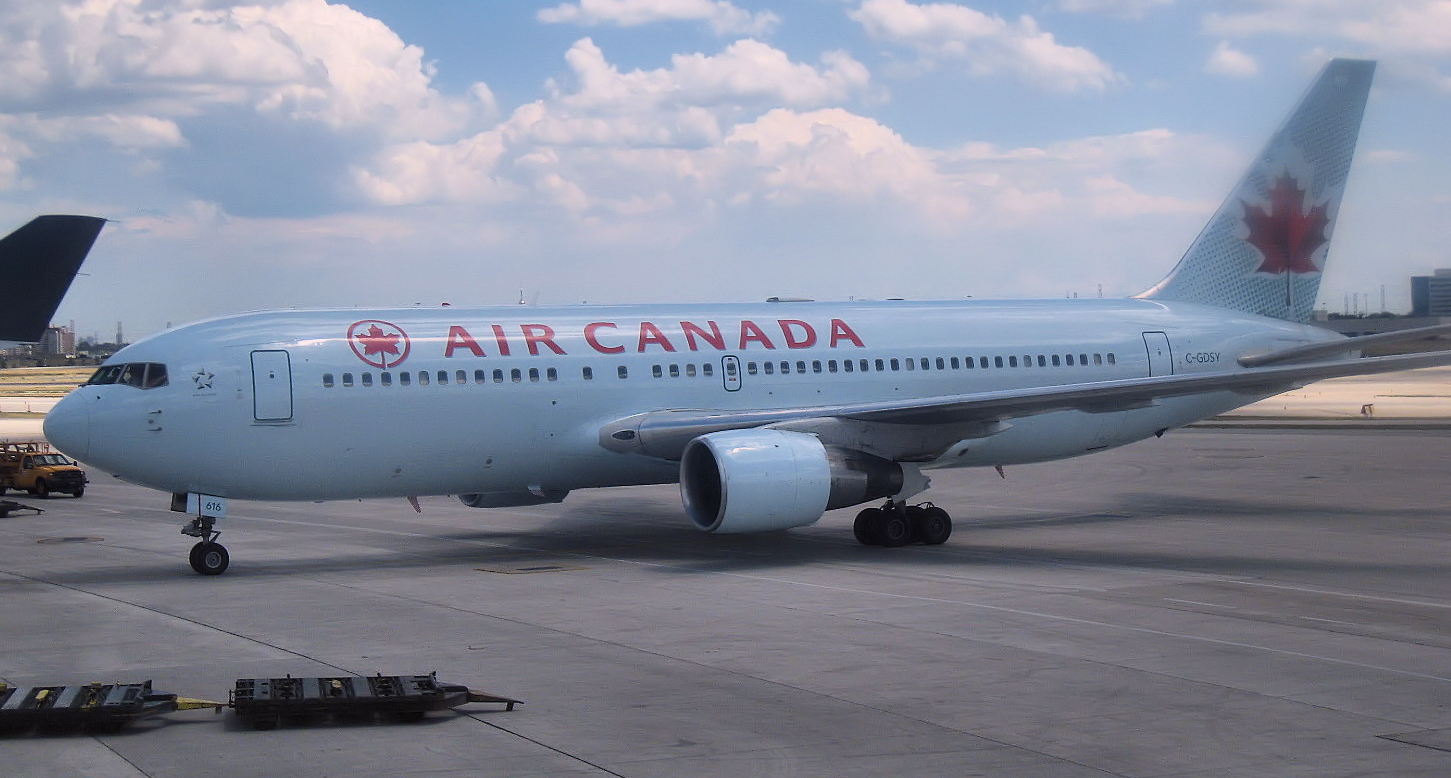
\includegraphics[width=1.1\columnwidth]{air-canada}
\end{frame}

\begin{frame}
  \vspace{-6pt}
  \hspace*{-.055\columnwidth}
  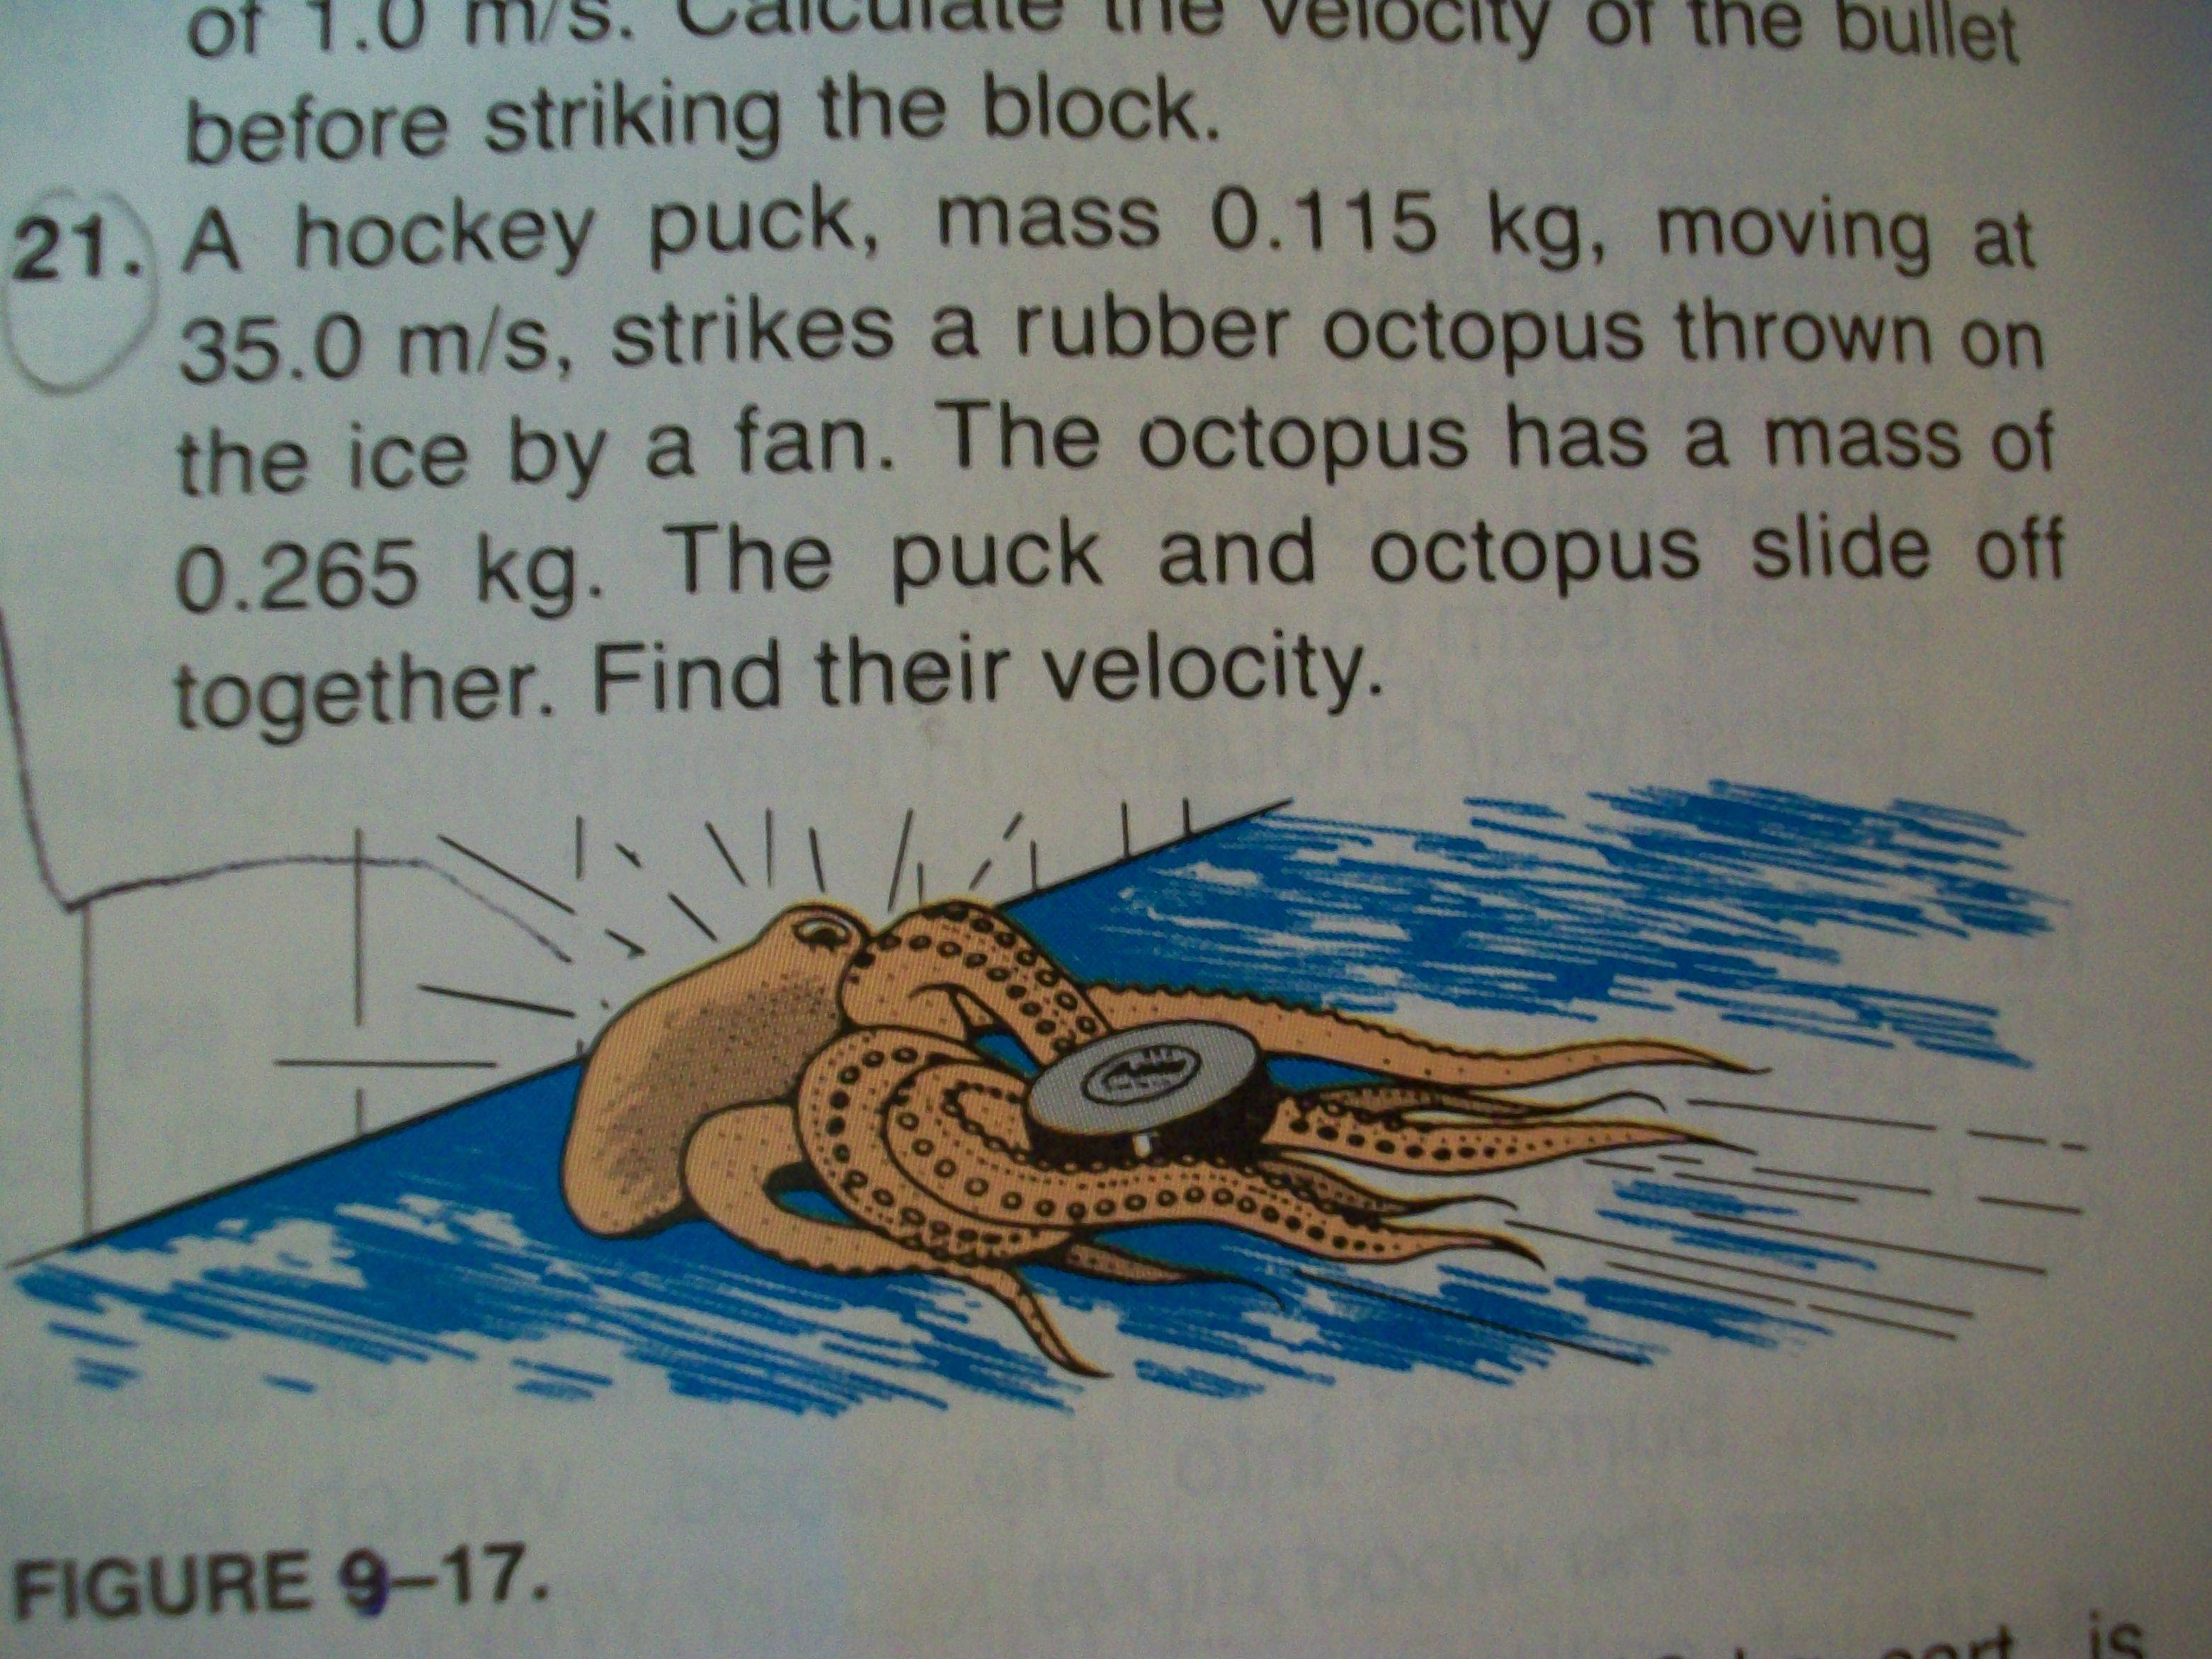
\includegraphics[width=1.15\columnwidth]{hockey-physics}
\end{frame}

\begin{frame}
  \vspace{-16pt}
  \begin{center}
    momentum before collision \\ = \\ momentum after collision \vspace{1.5em}

    momentum = mass ($m$) $\times$ velocity ($v$)
  \end{center}
\end{frame}

\begin{frame}
  \vspace{-40pt}
  \begin{align*}
    \onslide<1->{m_p v_p + m_o v_o &= (m_p + m_o) v_{po} \\ & \\}
    \onslide<2->{v_{po} &= \frac{m_p v_p + m_o v_o}{m_p + m_o} \\ & \\}
    \onslide<3->{v_{po} &= \frac{0.115 \times 35 + 0.265 \times 0.0}{0.115 + 0.265}} \\
    \onslide<3->{&= 10.5921052632}
  \end{align*}
\end{frame}

\begin{frame}[fragile]
  \vspace{-22pt}
  \begin{minted}{python}
mp = 0.115
vp = 35.0
mo = 0.265
vo = 0.0
v = (mp * vp + mo * vo) / (mp + mo)
# >>> print v
# 10.5921052632
  \end{minted}
\end{frame}

\begin{frame}[fragile]
  \vspace{-22pt}
  \begin{minted}{python}
mp = 0.115
vp = 114.13
mo = 0.265
vo = 0.0
v = (mp * vp + mo * vo) / (mp + mo)
# >>> print v
# 34.5393421053
  \end{minted}
\end{frame}

\begin{frame}[fragile]
  \vspace{-22pt}
  \begin{minted}{python}
mp = 0.115
vp = 114.13 * 0.44704  # mph to m/s
mo = 0.265
vo = 0.0
v = (mp * vp + mo * vo) / (mp + mo)
# >>> print v
# 15.4404674947
  \end{minted}
\end{frame}

\begin{frame}[fragile]
  \vspace{-22pt}
  \begin{minted}{python}
mp = 0.115  # kg
vp = 114.13 * 0.44704  # mph to m/s
mo = 0.265  # kg
vo = 0.0  # m/s
v = (mp * vp + mo * vo) / (mp + mo)
# >>> print v
# 15.4404674947
  \end{minted}
\end{frame}

\begin{frame}
  \vspace{-20pt}
  \begin{equation*}
    v_{po} = \frac{0.115 \,kg \times 35 \,m/s + 0.265 \,kg \times 0.0 \,m/s}
    {0.115 \,kg + 0.265 \,kg}
  \end{equation*}
\end{frame}

\begin{frame}
  \vspace{-12pt}
  Python packages
  \begin{itemize}
    \item \alert<2->{\texttt{quantities}}
    \item \texttt{unum}
    \item \texttt{buckingham}
    \item \texttt{magnitude}
    \item \texttt{piquant}
    \item \texttt{units}
    \item \texttt{dimpy}
  \end{itemize}
\end{frame}

\begin{frame}[fragile]
  \vspace{-22pt}
  \begin{minted}{python}
import quantities as pq
mp = 0.115 * pq.kg
vp = 35.0 * (pq.m / pq.s)
mo = 0.265 * pq.kg
vo = 0.0 * (pq.m / pq.s)
v = (mp * vp + mo * vo) / (mp + mo)
# >>> print v
# 10.5921052632 m/s
  \end{minted}
\end{frame}

\begin{frame}[fragile]
  \vspace{-22pt}
  \begin{minted}{python}
import quantities as pq
mp = 0.115 * pq.kg
vp = 114.13 * (pq.mi / pq.h)
mo = 0.265 * pq.kg
vo = 0.0 * (pq.m / pq.s)
v = (mp * vp + mo * vo) / (mp + mo)
# >>> print v
# 34.5393421053 mi/h
  \end{minted}
\end{frame}

\begin{frame}[fragile]
  \vspace{-22pt}
  \begin{minted}{python}
import quantities as pq
mp = 0.115 * pq.kg
vp = 114.13 * (pq.mi / pq.h)
mo = 0.265 * pq.kg
vo = 0.0 * (pq.m / pq.s)
v = (mp * vp + mo * vo) / (mp + mo)
# >>> print v.rescale(pq.km / pq.h)
# 55.5856829811 km/h
  \end{minted}
\end{frame}

\begin{frame}[fragile]
  \vspace{-22pt}
  \begin{minted}{python}
import quantities as pq
mp = 6.0 * pq.ounce
vp = 114.13 * (pq.mi / pq.h)
mo = 0.265 * pq.kg
vo = 0.0 * (pq.m / pq.s)
v = (mp * vp + mo * vo) / (mp + mo)
# >>> print v.rescale(pq.km / pq.h)
# 71.8057931081 km/h
  \end{minted}
\end{frame}

\begin{frame}
  \vspace{-20pt}
  \begin{align*}
    m/s &= \frac{kg \cdot m / s \alert{+ kg \cdot m / s}}{kg \alert{+ kg}} \\ & \\
    m/s &= \frac{\alert{kg} \cdot m / s}{\alert{kg}} \\ & \\
    m/s &= m/s
  \end{align*}
\end{frame}

\begin{frame}[fragile]
  \vspace{-22.5pt}
  \begin{minted}{python}
import quantities as pq
mp = 6.0 * pq.ounce
vp = 114.13 * (pq.mi / pq.h)
mo = 0.265 * pq.kg
vo = 0.0
v = (mp * vp + mo * vo) / (mp + mo)


  \end{minted}
\end{frame}

\begin{frame}[fragile]
  \vspace{-22pt}
  \begin{minted}{pycon}
Traceback (most recent call last):
  File "pucktopus-pq.py", line 8, in <>
    v = (mp * vp + mo * vo) / (mp + mo)
ValueError: Unable to convert between
units of "kg" and "oz*mi/h"
  \end{minted}
\end{frame}

\begin{frame}[fragile]
  \vspace{-12pt}
  \begin{center}
    \begin{minted}{python}
   pq.UnitQuantity(name, definition)


    \end{minted}
    \pause

    \begin{small}
      Suppose 250 people attend PyCon Canada. \\ ~ \\
      On average, each consumes 200 mL of milk.
    \end{small}
  \end{center}
\end{frame}

\begin{frame}
  \vspace{-4pt}
  How many bags of milk do we need? \vspace{1em}
  
  \hspace*{-.055\columnwidth}
  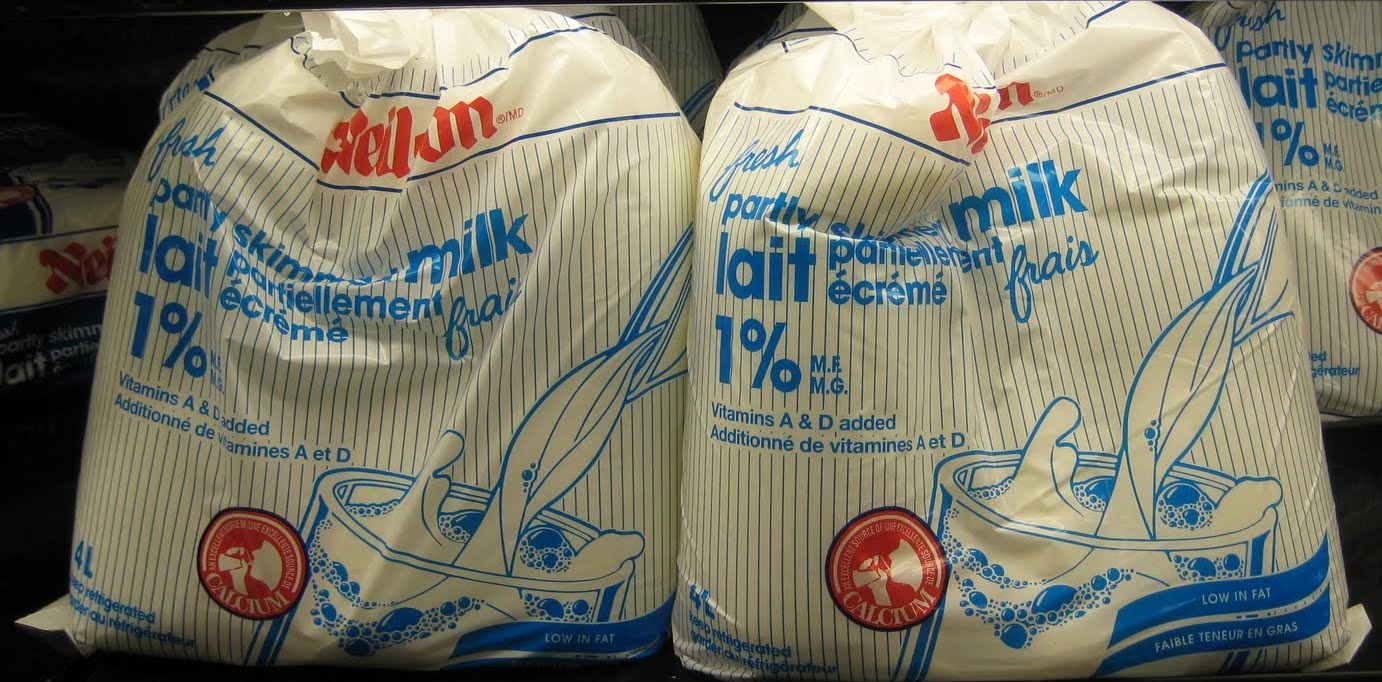
\includegraphics[width=1.1\columnwidth]{milkbags}
  % http://mini-angels.blogspot.ca/2011/05/my-canada-trip.html
  % http://2.bp.blogspot.com/-kNSbnHjjGd4/Tb33Y6JyJdI/AAAAAAAABGA/S6W_Zbg8kpE/s1600/IMG_1345.JPG
\end{frame}

\begin{frame}[fragile]
  \vspace{-22pt}
  \begin{minted}{python}
bags = pq.UnitQuantity('milk bags',
    pq.L * (4. / 3.))
person = pq.UnitQuantity('person',
    pq.dimensionless * 1)
need = 200 * (pq.mL / person)
need *= 250 * person
  \end{minted}
\end{frame}

\begin{frame}[fragile]
  \vspace{-8pt}
  \begin{minted}{pycon}
>>> print need
50000.0 mL
  \end{minted}
  \pause
  \begin{minted}{pycon}
>>> print need.rescale(pq.L)
50.0 L
  \end{minted}
  \pause
  \begin{minted}{pycon}
>>> print need.rescale(bags)
37.5 milk bags
  \end{minted}
  \pause
  \begin{minted}{pycon}
>>> import numpy as np
>>> print np.ceil(need.rescale(bags))
38.0 milk bags
  \end{minted}
\end{frame}

\begin{frame}
  \hspace*{-.055\columnwidth}
  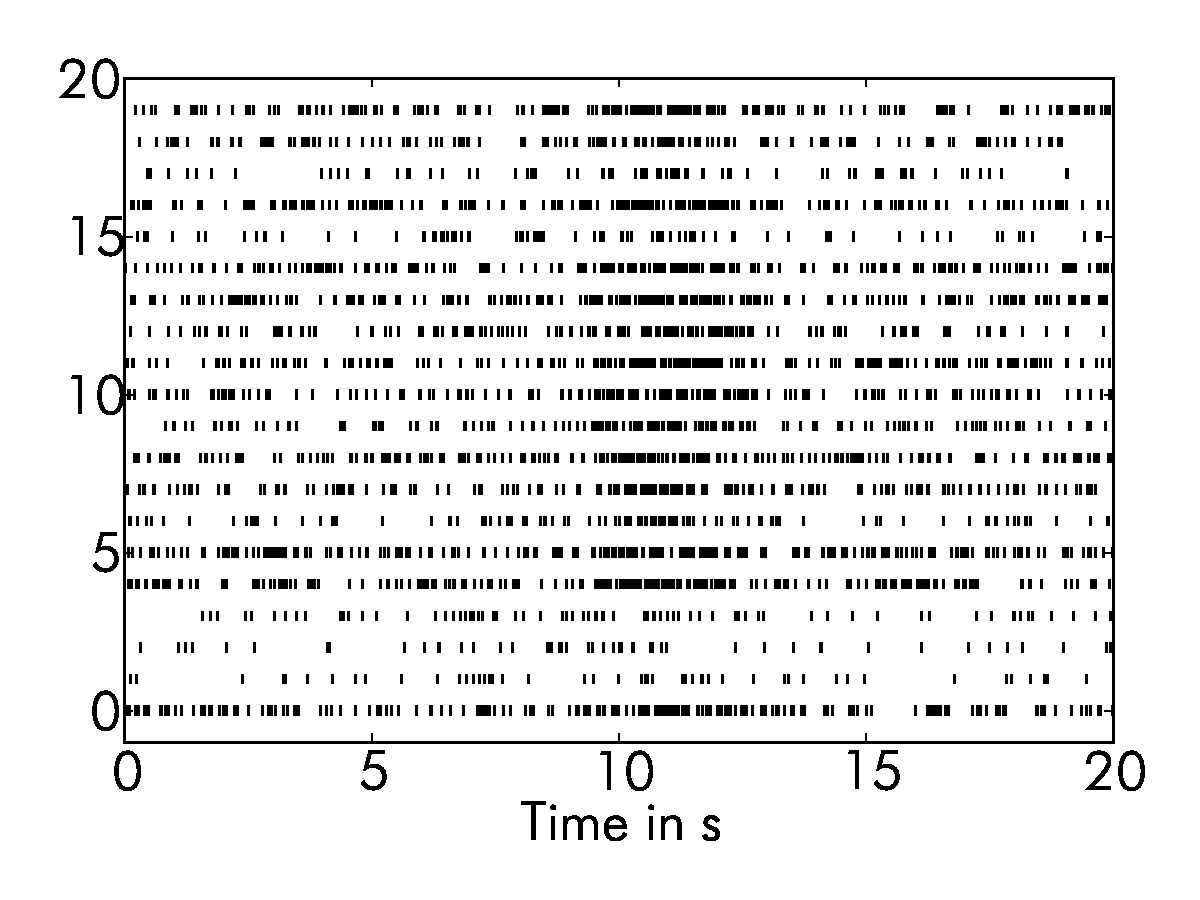
\includegraphics[width=1.1\columnwidth]{spikes-1}
\end{frame}

\begin{frame}
  \hspace*{-.055\columnwidth}
  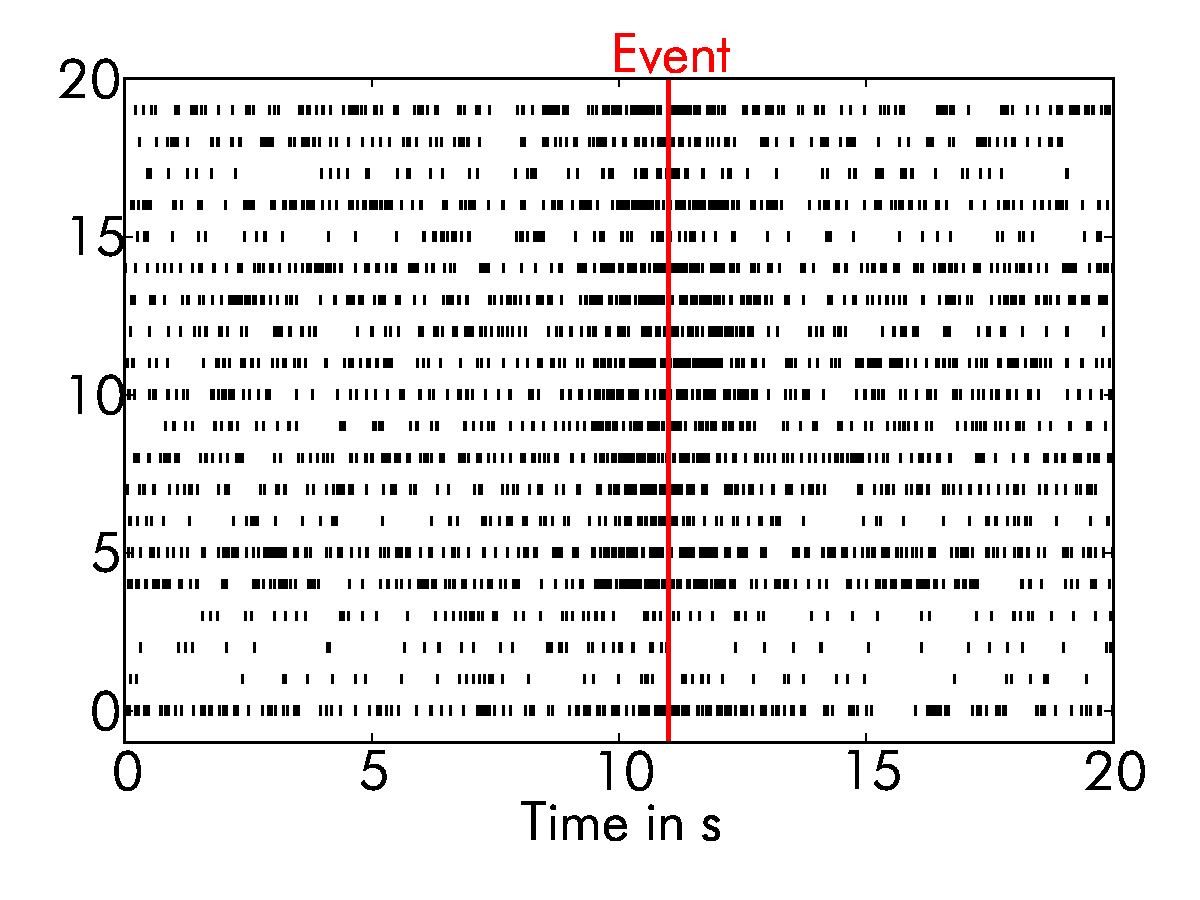
\includegraphics[width=1.1\columnwidth]{spikes-2}
\end{frame}

\begin{frame}
  \hspace*{-.055\columnwidth}
  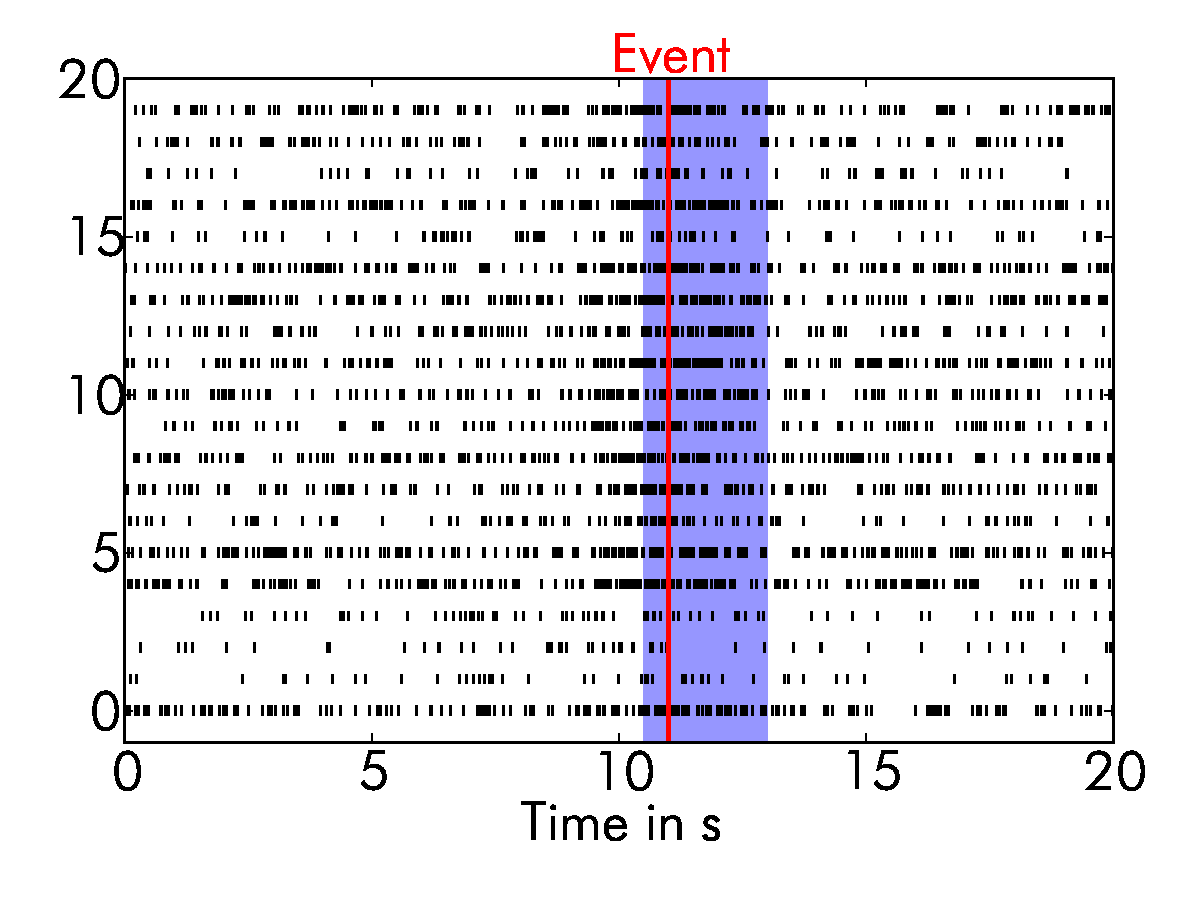
\includegraphics[width=1.1\columnwidth]{spikes-3}
\end{frame}

\begin{frame}
  \hspace*{-.055\columnwidth}
  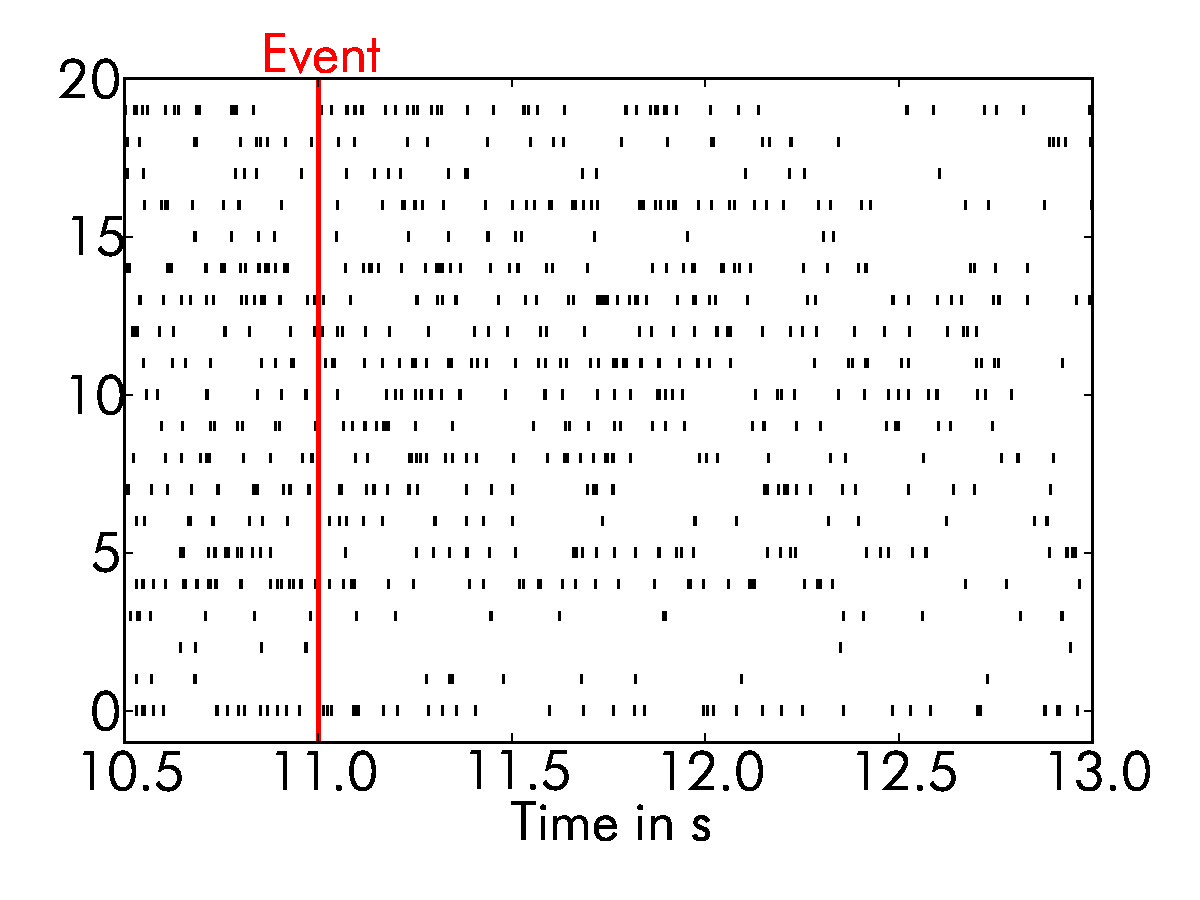
\includegraphics[width=1.1\columnwidth]{spikes-4}
\end{frame}

\begin{frame}
  \vspace{-22pt}
  \phantom{1. Seconds or milliseconds?}
  \texttt{spikes = load\_spikes('spikes.csv');}
  \vspace{16pt}

  \phantom{2. Bin size? Do we need to bin?}
  \texttt{binned = binspikes(spikes);}
  \vspace{16pt}

  \phantom{3. When is the actual event?}
  \texttt{perievent = spikes(525:650);}
\end{frame}

\begin{frame}
  \hspace*{-.055\columnwidth}
  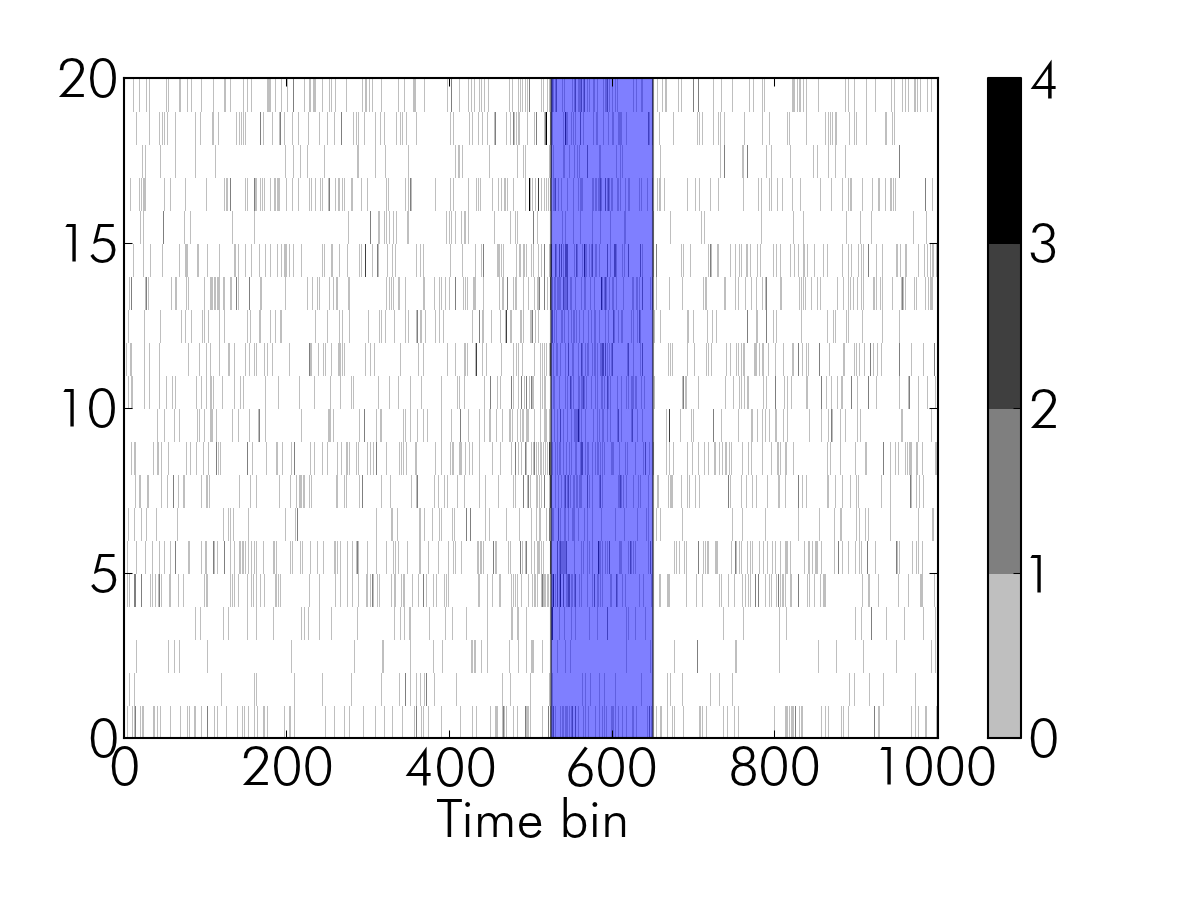
\includegraphics[width=1.1\columnwidth]{binned-1}
\end{frame}

\begin{frame}
  \hspace*{-.055\columnwidth}
  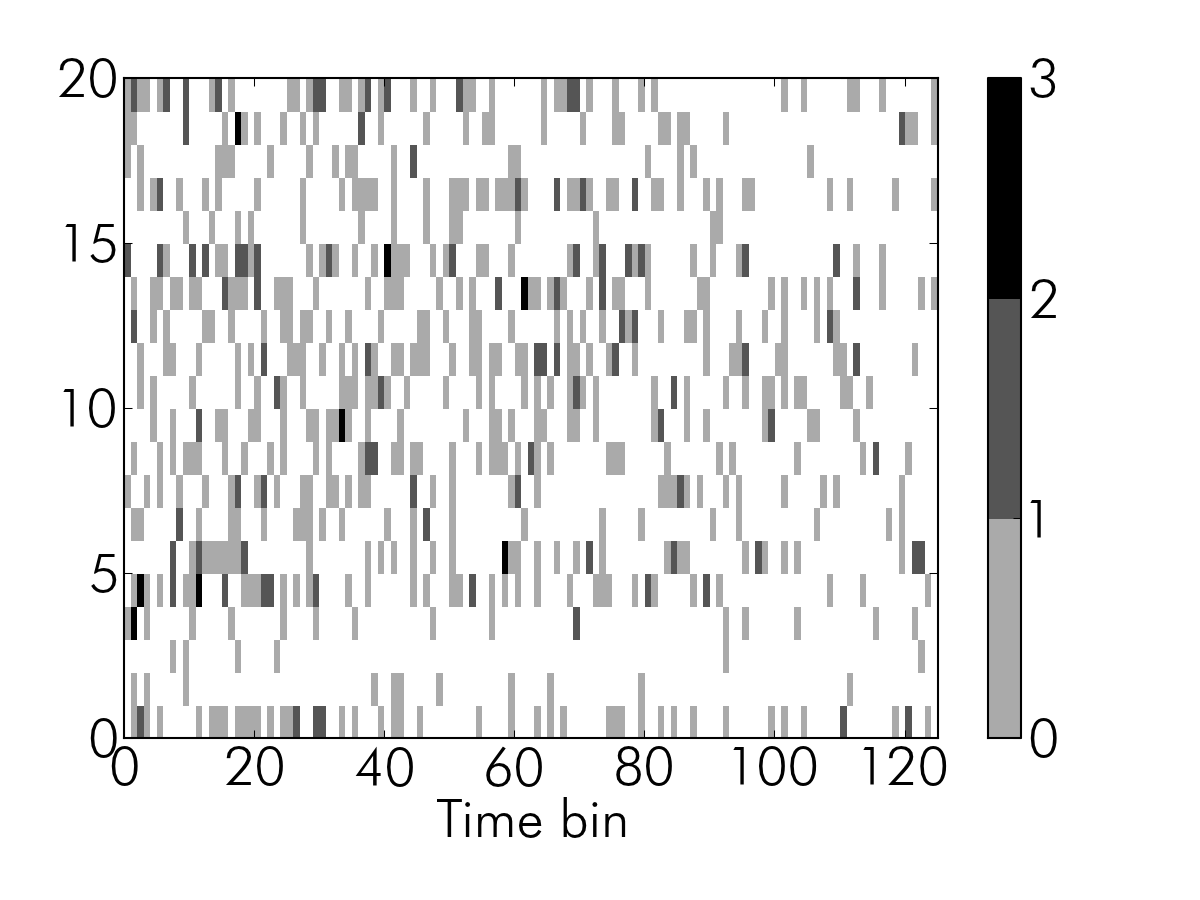
\includegraphics[width=1.1\columnwidth]{binned-2}
\end{frame}

\begin{frame}
  \vspace{-22pt}
  \onslide<2->{\alert<2>{1. Seconds or milliseconds?}} \\
  \texttt{spikes = load\_spikes('spikes.csv');}
  \vspace{16pt}

  \onslide<3->{\alert<3>{2. Bin size? Do we need to bin?}} \\
  \texttt{binned = binspikes(spikes);}
  \vspace{16pt}

  \onslide<4->{\alert<4>{3. When is the actual event?}} \\
  \texttt{perievent = spikes(525:650);}
\end{frame}

\begin{frame}[fragile]
  \vspace{-12pt}
  \begin{minted}{python}
spikes = (load_spikes('spikes.csv')
  * pq.s)
event = 11 * pq.s
window = (-0.5, 2) * pq.s
perievent = time_slice(spikes,
  *(event + window))
  \end{minted}
  \pause

  \begin{minted}{python}
def time_slice(spikes, tstart, tend):
    return spikes[np.logical_and(
      tstart <= spikes, spikes < tend)]
  \end{minted}
\end{frame}

\begin{frame}[fragile]
  \vspace{-12pt}
  \begin{minted}{python}
spikes = (load_spikes('spikes.csv')
  * pq.s).rescale(pq.ms)
event = 11 * pq.s
window = (-0.5, 2) * pq.s
perievent = time_slice(spikes,
  *(event + window))
  \end{minted}

  \begin{minted}{python}
def time_slice(spikes, tstart, tend):
    return spikes[np.logical_and(
      tstart <= spikes, spikes < tend)]
  \end{minted}
\end{frame}

\begin{frame}[fragile]
  \vspace{-12pt}
  \begin{small}
    \begin{minted}{python}
def bin_spikes(spikes, binsize, tstart, tend):
    binsize.units = tstart.units
    bins = np.arange(
      tstart, tend + binsize, binsize)
    return np.histogram(spikes, bins=bins)[0]

binned = bin_spikes(spikes, 20 * pq.ms,
  *(event + window))
    \end{minted}
  \end{small}
\end{frame}

\begin{frame}
   Try my code \\
  \begin{small}
    \url{https://github.com/tbekolay/pyconca2012}
  \end{small}\vspace{1em}

  Try out \texttt{quantities}! \\
  \texttt{~~~~pip install quantities} \\
  \texttt{~~~~easy\_install quantities} \\
  \begin{footnotesize}
    \url{http://packages.python.org/quantities/user/index.html}
  \end{footnotesize}\vspace{1em}

  \begin{large}
    Thank you!
  \end{large}
\end{frame}

\end{document}



